\documentclass[tikz,border=10pt]{standalone}
\usepackage{amsmath}
\usepackage{tikz}
\usetikzlibrary{arrows.meta, positioning}

\begin{document}
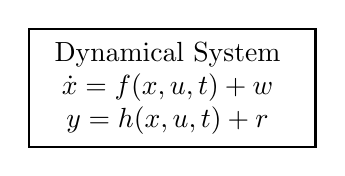
\begin{tikzpicture}[
    block/.style = {draw, thick, minimum height=2em, minimum width=4em, align=center},
    arrow/.style = {thick, -{Latex[width=2mm]}},
    node distance=1.8cm and 2.5cm
  ]

  % Nodes 
  \node[block] (system) {%
    \begin{tabular}{c}
      Dynamical System \\
      $\dot{x} = f(x,u,t) + w$ \\
      $y = h(x,u,t) + r$
    \end{tabular}
  };

\end{tikzpicture}
\end{document}
 
